\documentclass[manuscript,review]{acmart}

% --- Required Package Configurations ---
\usepackage{booktabs} % For professional tables
\usepackage{graphicx} % For enclosing screenshots if necessary
\usepackage{enumitem}

% --- ACM Citation & Bibliography Styles ---
\citestyle{acmauthoryear} % Sets up ACM citation format

% --- Paper Header Metadata (Exact Match) ---
\title{RepairAgent: An Autonomous, LLM-Based Agent for Program Repair}

\author{Islem Bouzenia}
\email{fi\_bouzenia@esi.dz}
\affiliation{%
  \institution{University of Stuttgart}
  \country{Germany}
}

\author{Premkumar Devanbu}
\email{ptdevanbu@ucdavis.edu}
\affiliation{%
  \institution{UC Davis}
  \country{USA}
}

\author{Michael Pradel}
\email{michael@binaervarianz.de}
\affiliation{%
  \institution{University of Stuttgart}
  \country{Germany}
}

% --- Main Document Content ---
\begin{document}

\begin{abstract}
Automated program repair has emerged as a powerful technique to mitigate the impact of software bugs on system reliability and user experience. This paper introduces RepairAgent, the first work to address the program repair challenge through an autonomous agent based on a large language model (LLM). Unlike existing deep learning-based approaches, which prompt a model with a fixed prompt or in a fixed feedback loop, our work treats the LLM as an agent capable of autonomously planning and executing actions to fix bugs by invoking suitable tools. Repair Agent freely interleaves gathering information about the bug, gathering repair ingredients, and validating fixes, while deciding which tools to invoke based on the gathered information and feedback from previous fix attempts. Key contributions that enable RepairAgent include a set of tools that are useful for program repair, a dynamically updated prompt format that allows the LLM to interact with these tools, and a finite state machine that guides the agent in invoking the tools. Our evaluation on the popular Defects4J dataset demonstrates RepairAgent's effectiveness in autonomously repairing 164 bugs, including 39 bugs not fixed by prior techniques. Interacting with the LLM imposes an average cost of 270k tokens per bug, which, under the current pricing of OpenAl's GPT-3.5 model, translates to 14 cents per bug. To the best of our knowledge, this work is the first to present an autonomous, LLM-based agent for program repair, paving the way for future agent-based techniques in software engineering.
\end{abstract}

\maketitle

\section{Introduction}
% TODO: Summarize the introduction in your own words.
% Mention the shift from traditional APR to 1st/2nd-generation LLM loops, 
% and contrast it with RepairAgent's human-like interleaving actions.
Software bugs can lead to system failures, security vulnerabilities, and compromised user experience. Manually fixing bugs demands significant time and user effort, but \textbf{A}utomated \textbf{P}rogram \textbf{R}epair (APR) can significantly reduce the effort via automatic bug resolution. Various approaches have been explored in this regard \cite{legoues2019automated}, incl. techniques based on manually designed \cite{legoues2012genprog}, \cite{liu2019tbar} and (semi-)automatically extracted \cite{kim2013automatic}, \cite{bader2019getafix} fix patterns, based on symbolic constraints \cite{nguyen2013semfix}, \cite{xuan2016nopol}, and various machine learning based approaches \cite{long2016automatic}, \cite{gupta2017deepfix}, \cite{tufano2019learning}. \newline
The current state-of-the-art in APR is predominated by LLMs. In the first generation of LLM based APR, the model expects a prompt with the buggy code and produces the fixed version \cite{xia2023automated}, \cite{jiang2023impact}, but further development introduces an iterative aproach: the LLM is queried repeatedly based on feedback obtained from previous fix attempts \cite{xia2023keep}, \cite{kang2023explainable}, \cite{ye2024iter}.\newline
But this approach has a few limitations since the hard-coded feedback loops in the LLMs do not allow them to gather information about existing bugs or existing code that may provide them with debugging ingredients, unlike manual human debugging which typically incorporates a temporal interleaving of gathering information to gain understanding of the bug, searching code that might help in debugging and then attempting various versions of fixes \cite{ko2006exploratory}, \cite{bohme2017where}.\newline
This paper represents \textbf{RepairAgent}, the first autonomous, LLM based agent for automated program repair. The LLM is treated as an autonomous agent capable of planning and executing actions to fix a bug. The LLM is equipped with a set of repair-specific tools. How and when to use these tools aren't hard coded, rather the LLM gets to autonomously decide. \newline
The approach is enabled via three key components: a general purpose LLM e.g. GPT-3.5, a set of tools for the LLM to use (in this approach, 14 tools in total have been used), and a middleware to establish communication between the tools and the LLM.\newline
The novelty of the approach was tested using all 835 bugs of the Defects4J \cite{just2014defects4j} dataset. 164 bugs were successfully fixed, including 39 bugs that were not fixed by prior state-of-the-art work \cite{xia2023keep} \cite{ye2024iter}. \newline
The interaction with the LLM imposes a cost of ~270K tokens per bug on average, which translates to about \textbf{14 cents} per bug. \newline
In summary, this paper contributes the following:
\begin{itemize}
  \item An autonomous, LLM-based agent for program repair.
  \item A dynamically updated prompt format that guides the LLM through the bug repair process.
  \item A set of tools that enable a LLM to to perform steps a human developer would take when fixing a bug.
  \item A middleware that guides via a finite state machine how the LLM interacts with the tools.
  \item Empirical evidence that RepairAgent establishes a new state of the art in program repair.
  \item We release our implementation as open-source: \url{https://github.com/sola-st/RepairAgent}.
\end{itemize}
\noindent To the best of our knowledge, this is the first work to present an autonomous, LLM-based agent for program repair, paving the way for future agent-based techniques in software engineering.



\section{Background (LLM-Based Autonomous Agents)}
Because of extensive training, LLMs have demonstrated remarkable abiliteies in in achieving human-level performance in a variety of tasks \cite{bubeck2023sparks}. A promising way to use these LLMs are LLM-based agents, which mean LLM-based techniques with two properties: (1) The LLM can autonomously plan for and execute a set of actions to acheive a particular goal, unlike hard-coded algorithmic processes, and (2) The actions by the LLM can invoke external tools, enabling it to interact with its environment \cite{schick2023toolformer} \cite{patil2023gorilla}. In the context of Software Engineering, the tools could be tools usually used by developers, e.g., as part of an integrated development environment (IDE). Basically, we query the LLM with the current state of the world, the goal and a set of actions to perform. The feedback is integrated into the next prompt. 

\section{Method}

\subsection{Overview}
Fig. 1 provides an overview of RepairAgent. 

\begin{figure}[h]
\centering
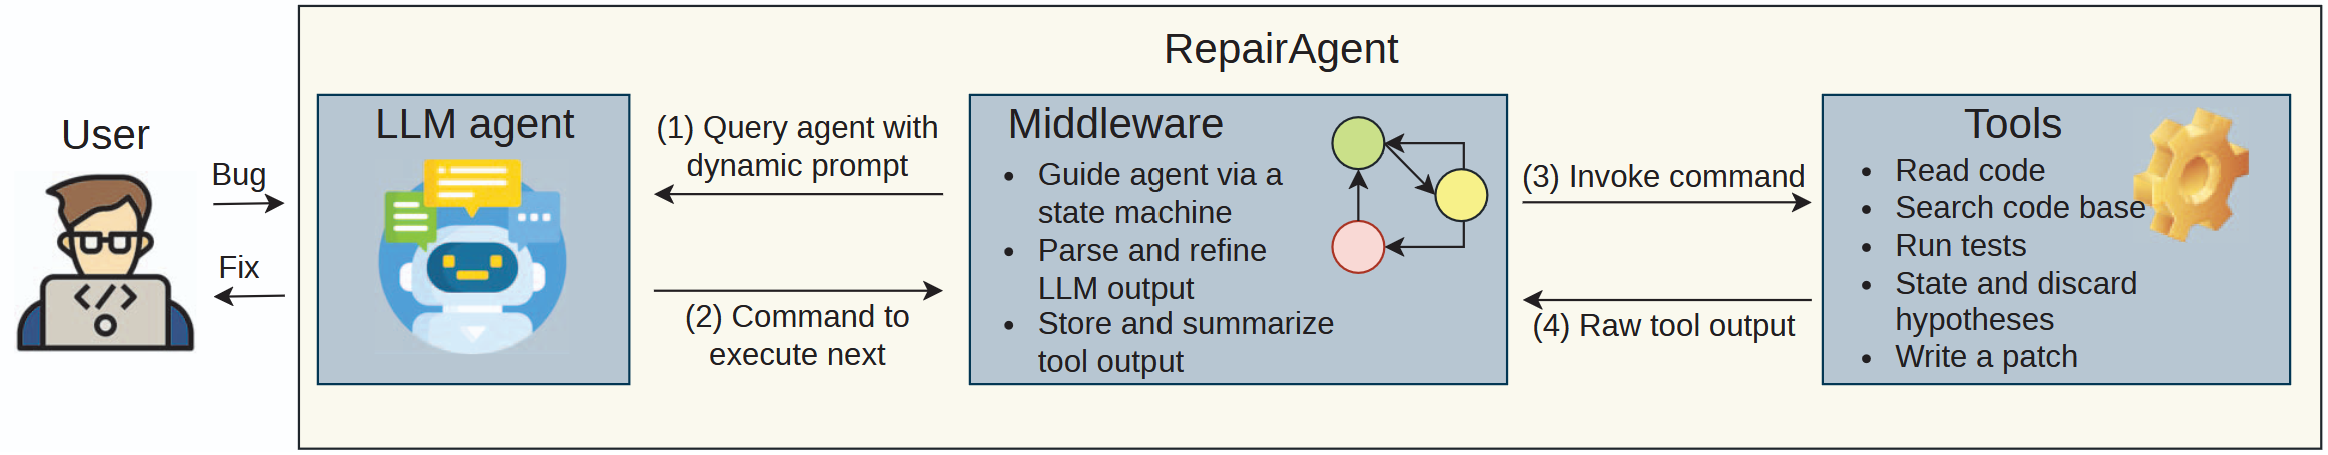
\includegraphics[width=0.9\linewidth]{fig_1.png}
\caption{Overview of RepairAgent.}
\label{fig_1}
\end{figure}

\subsection{Terminology}
RepairAgent proceeds in multiple cycles:

\noindent \textbf{Definition 1} (Cycle). A \textit{cycle} represents one round of interaction with the LLM agent, which consists of the following steps:
\begin{enumerate}
    \item Query the agent
    \item Post-process the response
    \item Execute the command suggested by the agent
    \item Update the dynamic prompt based on the command's output
\end{enumerate}

\noindent In each cycle, the approach queries the LLM once. The input to the model is updated based on commands invoked by the LLM, and their results, in previous cycles. We call the model input a dynamic prompt: \newline
\noindent \textbf{Definition 2} (Dynamic prompt). The \textit{dynamic prompt} is a sequence of text sections $P = [s_0, s_1, \dots, s_n]$, where each section $s_i$ is one of the following (where $s_i(c)$ refers to a section during a cycle $c$):
\begin{itemize}
    \item A \textit{static section}, which remains the same across all cycles, i.e., $s_i(c) = s_i(c')$ for all $c, c'$.
    \item A \textit{dynamic section}, which may differ across cycles, i.e., there may exist $c, c'$ with $s_i(c) \neq s_i(c')$.
\end{itemize}

\subsection{Dynamic Prompting of the RepairAgent}
As listed in Table 1, the prompt contains multiple static and dynamic sections.

\begin{table}[h]
\caption{Sections of the dynamically updated prompt within RepairAgent}
\label{tab:prompt_sections}
\centering
\begin{tabular}{ll}
\toprule
\textbf{Prompt Section} & \textbf{Nature} \\
\midrule
Role & Static \\
Goals & Static \\
Guidelines & Static \\
State description & Dynamic \\
Available tools & Dynamic \\
Gathered information & Dynamic \\
Specification of output format & Static \\
Last executed command and result & Dynamic \\
\bottomrule
\end{tabular}
\end{table}

\noindent \textbf{(1) Role}: provides the agent's area of expertise and outlines the agent's primary objective: finding and fixing bugs \newline
\textbf{(2) Goals}: There are \textbf{5 goals} for the agent to pursue:
\begin{enumerate}[label=\alph*)]
  \item \textit{Locate the bug} using testing and fault localization techniques
  \item \textit{Gather information about the bug} by analyzing the relevant portion(s) of the codebase
  \item \textit{Suggest simple fixes to the bug} 
  \item \textit{Suggest complex fixes} 
  \item \textit{Iterate over the previous goals}
\end{enumerate}
\noindent \textbf{(3) Guidelines}: The LLM is provideed with a set of guidelines. It is told that there are various kinds of bugs ranging from one-line-fix bugs to multi-line bugs. A list of recurring fix patterns is also provided that help solve many common bugs \cite{karampatsis2020how} which is based on single-statement bugs in \textbf{Java}. The model is also instructed to add comments along with edited code which helps the model explain its reasoning and improve itself \cite{wei2022chain}. The model is also instructed to define a next step that can be converted into a call to a tool. \newline 
\noindent \textbf{(4) State description}: To guide the LLM toward using the tools effectively, a state machine is defined that constrains which tool(s) can be used at any given time. This is to stop the LLM to get lost in aimless exploration, which has happened very frequently as per the results of earlier tests. Fig. 2 shows the finite state machine. The set of tools are described in Section 3.4. The agent is free to move between any state via tools.
\begin{figure}[h]
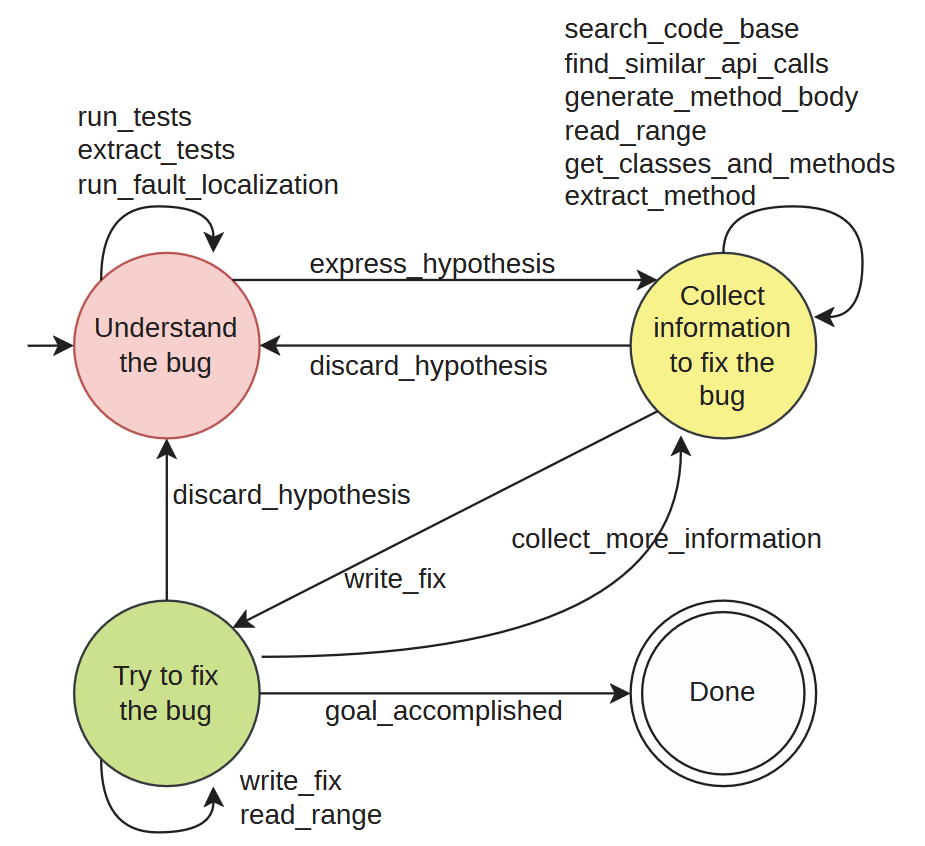
\includegraphics[width=0.5\textwidth]{fig_2.png}
\caption{State machine to guide selection of tools.}
\label{fig_2}
\end{figure}  \newline
\begin{itemize}
  \item \textit{Understand the bugs}: The agent can collect information and bug location from testing results. It can then formulate a hypothesis based on its knowledge.
  \item \textit{Collect information to fix the bug}: The agent can search for specific repair methods or read relevant code. After gathering enough informaton, it moves on to the next state.
  \item \textit{Try to fix the bug}: The agent can try to fix the bug based on the hypothesis and information gathereed. If necessary, the agent can go back and establish a new hypothesis or gather additional information. 
\end{itemize}
\noindent \textbf{(5) Available tools}:  \newline
\noindent \textbf{(6) Gathered information}:  \newline
\noindent \textbf{(7) Specification of output format}:  \newline 
\noindent \textbf{(8) Last executed command and result}:  \newline


\section{Findings/Results}
% TODO: Summarize findings on Defects4J, GitBug-Java, costs, and the ablation study.
Evaluations performed across the Defects4J benchmark indicate that RepairAgent effectively resolved 164 functional bugs, establishing capabilities beyond baseline tools like ChatRepair and ITER \cite{defects4j, chatrepair, iter}. This performance is especially visible in multi-line fixes due to the contextual integration of search features \cite{repairagent}. Financial evaluations tracking token tracking usage configurations show an average financial overhead of approximately 14 cents per bug resolution attempt under standard model frameworks \cite{repairagent}. Further cross-validation against the GitBug-Java set shows functional adaptation across varied setups \cite{gitbugjava}.

\section{Discussion}
% TODO: Summarize qualitative insights and threats to validity (data leakage, etc.)
Qualitative tracing indicates that access to structural tools yields better insights into functional anomalies \cite{repairagent}. However, complex modifications sometimes introduce unintended changes to straightforward single-line defects. Threats to internal and external validity include data leakage concerns during foundational model pre-training steps and reliance on highly precise localized metrics generated via secondary spectrum coverage frameworks like GZoltar \cite{gzoltar}.

% --- References Section ---
\bibliographystyle{ACM-Reference-Format}
\bibliography{references}

\end{document}